\documentclass{beamer}
\usepackage{pxfonts}
\usepackage{tikz}
\usepackage{ifthen}



\usetikzlibrary{calc,shadows}


\mode<presentation>
\usetheme[height=.75cm]{Rochester}

\title{GIT}
\author{Fr\'ed\'eric Vogels}
\institute[KHL]{KHLeuven}


\pgfkeys{
  /tikz/.cd,
  file/.style={fill=red!50,minimum width=.75cm,font=\tiny,draw},
  blob/.style={draw,fill=blue!50,font=\tiny,inner sep=.5mm},
  link/.style={-latex},
  note/.style={fill=gray!50,draw,drop shadow},
  note arrow/.style={->},
  caption/.style={fill=gray!50,draw,drop shadow,font={\Huge\sc}},
  command/.style={fill=gray!50,draw,font={\tt\small}},
  data area/.style={fill=blue!25,minimum width=10cm,minimum height=1cm,text opacity=.25,font={\Huge\sc\color{blue}}},
  working directory/.style={fill=red!25,minimum width=10cm,minimum height=1cm,text opacity=.25,font={\Huge\sc\color{red}}},
  staging area/.style={fill=orange!25,minimum width=10cm,minimum height=1cm,text opacity=.25,font={\Huge\sc\color{orange}}},
  repository/.style={fill=green!25,minimum width=10cm,minimum height=1cm,text opacity=.25,font={\Huge\sc\color{green}}},
}

\newcommand{\bits}[1]{
  {
    \pgfmathparse{bin(128+mod(#1 * 229 + 73, 128))}\let\x\pgfmathresult
    \pgfmathparse{bin(128+mod(#1 * 541 + 111, 128)}\let\y\pgfmathresult
    \parbox{.9cm}{\centering\tt \x \\ \y}
  }
}

\newcommand{\dataarea}{\node[data area,anchor=north] at (0,0) {data area};}
\newcommand{\workingdirectory}{\node[working directory,anchor=south] at (0,0) {working directory};}
\newcommand{\stagingarea}{\node[staging area,anchor=south] at (0,1) {staging area};}
\newcommand{\repository}{\node[repository,anchor=south] at (0,2) {repository};}

\newcommand{\CAPTION}[1]{\node[caption] (caption) at (0, -3.5) {#1};}
\newcommand{\COMMAND}[1]{\node[command] at (0,-2.5) {#1};}

\begin{document}

\titlepage

\section{Without Version Control}

\frame{\tableofcontents[currentsection]}

\begin{frame}
  \frametitle{Without Version Control}
  \begin{center}
    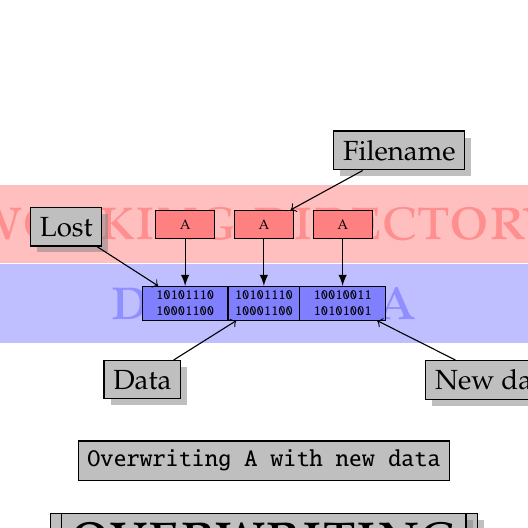
\begin{tikzpicture}
      \path[use as bounding box] (-3,-3) rectangle (3,3);
      \dataarea
      \workingdirectory

      \onslide<2>{
        \COMMAND{Creation of file A}
      }

      \onslide<2-3>{
        \node[blob] (x) at (0,-.5) {\bits{1}};
        \node[file] (A) at ($ (x) + (0,1) $) {A};
        \draw[link] (A) -- (x);
        \CAPTION{file creation}
      }

      \onslide<3>{
        \node[note,anchor=south west] (note A) at ($ (A.north east) + (.5,.5) $) {Filename};
        \draw[note arrow] (note A) -- (A);

        \node[note,anchor=north east] (note x) at ($ (x.south west) + (-.5,-.5) $) {Data};
        \draw[note arrow] (note x) -- (x);
      }

      \onslide<4-7>{
        \CAPTION{overwriting}
      }

      \onslide<5>{
        \COMMAND{Overwriting A with new data}
      }

      \onslide<4-6>{
        \node[blob] (x) at (-1,-.5) {\bits{1}};
      }
      \onslide<4>{
        \node[file] (A) at ($ (x) + (0,1) $) {A};
        \draw[link] (A) -- (x);
      }
      \onslide<5-7>{
        \node[blob] (y) at ($ (x) + (2,0) $) {\bits{2}};
        \node[file] (A) at ($ (y) + (0,1) $) {A};
        \draw[link] (A) -- (y);
      }
      \onslide<6>{
        \node[note,anchor=south east] (note x) at ($ (x.north west) + (-.5,.5) $) {Lost};
        \draw[note arrow] (note x) -- (x);

        \node[note,anchor=north west] (note y) at ($ (y.south east) + (.5,-.5) $) {New data};
        \draw[note arrow] (note y) -- (y);
      }
    \end{tikzpicture}
  \end{center}
\end{frame}

\section{Staging Area}

\frame{\tableofcontents[currentsection]}

\begin{frame}
  \frametitle{Staging Area}
  \begin{center}
    \begin{tikzpicture}
      \path[use as bounding box] (-3,-3) rectangle (3,3);

      \dataarea
      \workingdirectory
      \stagingarea

      \only<1-4>{
        \CAPTION{add operation}
      }
        
      \only<1->{
        \node[blob] (x) at (-1,-.5) {\bits{1}};
      }

      \only<1-3>{
        \node[file] (A) at ($ (x) + (0,1) $) {A};
        \draw[link] (A) -- (x);
      }

      \only<2>{
        \COMMAND{git add A}
      }

      \only<2->{
        \node[file] (working A) at ($ (A) + (1,1) $) {A};
        \draw[link] (working A) -- (x);
      }

      \only<3>{
        \node[note,anchor=south west] (working A note) at ($ (working A.north east) + (.5,.5) $) {copy};
        \draw[note arrow] (working A note) -- (working A);
      }

      \only<4>{
        \COMMAND{We overwrite A}
      }

      \only<4->{
        \node[blob] (y) at (1,-.5) {\bits{2}};
        \node[file] (A2) at ($ (y) + (0,1) $) {A};
      }

      \only<4-5>{
        \draw[link] (A2) -- (y);
      }

      \only<5->{
        \CAPTION{checkout operation}
      }

      \only<6>{
        \COMMAND{git checkout A}
      }

      \only<6->{
        \draw[link] (A2) -- (x);
      }

      \only<7>{
        \node[note,anchor=south west] (note A2) at ($ (A2.north east) + (.5,.5) $) {Old version restored};
        \draw[note arrow] (note A2) -- (A2);
      }
    \end{tikzpicture}
  \end{center}
\end{frame}

\begin{frame}
  \frametitle{Staging Area}
  \begin{itemize}
    \item Keeps a simple copy of the working directory
    \item {\tt add}: copy current version to staging area
    \item {\tt checkout}: restore to version in staging area
    \item No versioning
    \item Rudimentary backup system
  \end{itemize}
\end{frame}

\end{document}



%%% Local Variables: 
%%% mode: latex
%%% TeX-master: t
%%% End: 
